%%%%%%%%%%%%%
\begin{singlespace}
\section{Aplication to Synthetic Data}

\noindent{In order to test the efficiency of the proposed inversion method, we applied it to two sets of synthetic data contaminated by high and/or low frequency noise. }

\noindent{The first synthetic test is performed by generating a simple set of four spheres with similar magnetization intensity and radius, but completely different magnetization directions. Generating a data set contaminated by high frequency noise. In this simulation, the magnetization directions and magnetic moment intensity are directly compared with the initial input parameters. This first simplified test is basically done to investigate the efficiency of the inversions used for Euler positioning and magnetization parameters, thus being a validation of the methodology.}

\noindent{The second data set is data generated by a more complex model containing one hundred spheres with different radius and magnetization intensity, but magnetized in a similar direction within one standard deviation. This data set is corrupted by both low and high frequency noise. In this second application there is also validation using the comparison of the model data with the retrieved data. The complexity of this synthetic data seeks to more faithfully simulate the applicability of the proposed method to real SMM data.}


%%%
\subsection{Simple Simulation: Validating the Methodology}

\noindent{We applied the proposed method in a numerical simulation of a geological thin-section of dimensions 1000 μm x 1000 μm in a regular grid (1000 x 1000) for estimating the magnetization directions of four spherical sources uniformly magnetized (but with different directions), according to \cref{tab:SimpleSyntheic}. Totaling an observation number N = $10^6$ obtained at a sensor-sample distance of 5 μm and a grid spacing of 1 μm. Subsequently, the data vector was contaminated with a pseudo-random noise of normal Gaussian distribution with a zero mean and 15 nT standard deviation, as shown in \cref{fig:SimpleSynthetic}a.}

\bigskip

\floatsetup[table]{capposition=top} % to put the caption on the top of the table
% If you use beamer only pass "xcolor=table" option, i.e. \documentclass[xcolor=table]{beamer}

\begin{table}[htbp]
\caption{Each source positioning and magnetization parameters modelled and recovered using least square estimator, respectively.}
\label{tab:SimpleSyntheic}
\resizebox{1.0\textwidth}{!}{
\begin{tabular}{ccccccc}
\hline   
\rowcolor[HTML]{FFFFFF} 
\cellcolor[HTML]{FFFFFF}                         & \multicolumn{3}{c}{\cellcolor[HTML]{FFFFFF}Center coordinates} & \multicolumn{3}{c}{\cellcolor[HTML]{FFFFFF}Magnetization}    \\
\rowcolor[HTML]{FFFFFF} 
\multirow{-2}{*}{\cellcolor[HTML]{FFFFFF}Sphere} & Xc ($\mu   m$)     & Yc ($\mu   m$)     & Zc ($\mu   m$)    & m ($A \cdot m^2$)       & D (\textdegree)          & I (\textdegree)           \\  \hline 
\multirow{2}{*}{1}                               & 250.00                 & 250.00                 & 5.30                & \multicolumn{1}{l}{8.70e-15}  & \multicolumn{1}{l}{-140.00}   & \multicolumn{1}{l}{-30.00}    \\ 
                                                 & 250.28                 & 250.19                 & 5.38                & 8.82e-15  $\pm$  1.39e-17           & -140.22  $\pm$  0.11            & -30.04    $\pm$  0.08           \\  \hline 
\multirow{2}{*}{2}                               & 500.00                 & 500.00                 & 7.75                & \multicolumn{1}{l}{7.63e-15}  & \multicolumn{1}{l}{-70.00}   & \multicolumn{1}{l}{-50.00}    \\ 
                                                 & 500.46                 & 500.50                 & 7.77                & 7.67e-15  $\pm$  1.90e-17           & -69.42  $\pm$  0.26            & -49.85    $\pm$  0.15           \\  \hline 
\multirow{2}{*}{3}                               & 750.00                 & 750.00                 & 8.50                & \multicolumn{1}{l}{6.21e-15}  & \multicolumn{1}{l}{10.00}   & \multicolumn{1}{l}{62.00}    \\
                                                 & 750.73                 & 750.72                 & 8.57                & 6.31e-15  $\pm$  1.99e-17           & 9.06  $\pm$  0.50            & 62.34    $\pm$  0.22           \\  \hline 
\multirow{2}{*}{4}                               & 200.00                 & 800.00                 & 10.00                & \multicolumn{1}{l}{4.97e-15}  & \multicolumn{1}{l}{125.00}   & \multicolumn{1}{l}{22.00}    \\
                                                 & 200.30                 & 800.92                 & 10.00                & 4.94e-15  $\pm$  3.01e-17           & 124.63  $\pm$  0.39            & 21.76    $\pm$  0.27           \\  \hline
\end{tabular}
}
\end{table}




\bigskip

\noindent{The first step is to apply the upward continuaton filter, which transforms the potencial field measured on a surface into one measured at a higher surface level \citep{Blakely1996}, therefore smoothing out high frequency noise. This first step is always needed in high frequency noisy data, since the Euler equation requires the first derivatives of potencial field. If this step is negleted or badly elaborated, the high frequency noise propagation during the application of the derivative filters will cause future errors in the next methodological stage.} 

\noindent{The next step is to calculate the magnetic total gradient (or horizontal gradient) filter in order to highlight the anomaly signal of each source within its own boundaries, then we apply the blob detection algorithm \citep{VanderWalt2014} to obtain a robust positioning of each source data window (\cref{fig:SimpleSynthetic}b).}

\begin{figure}[htbp]
\centering
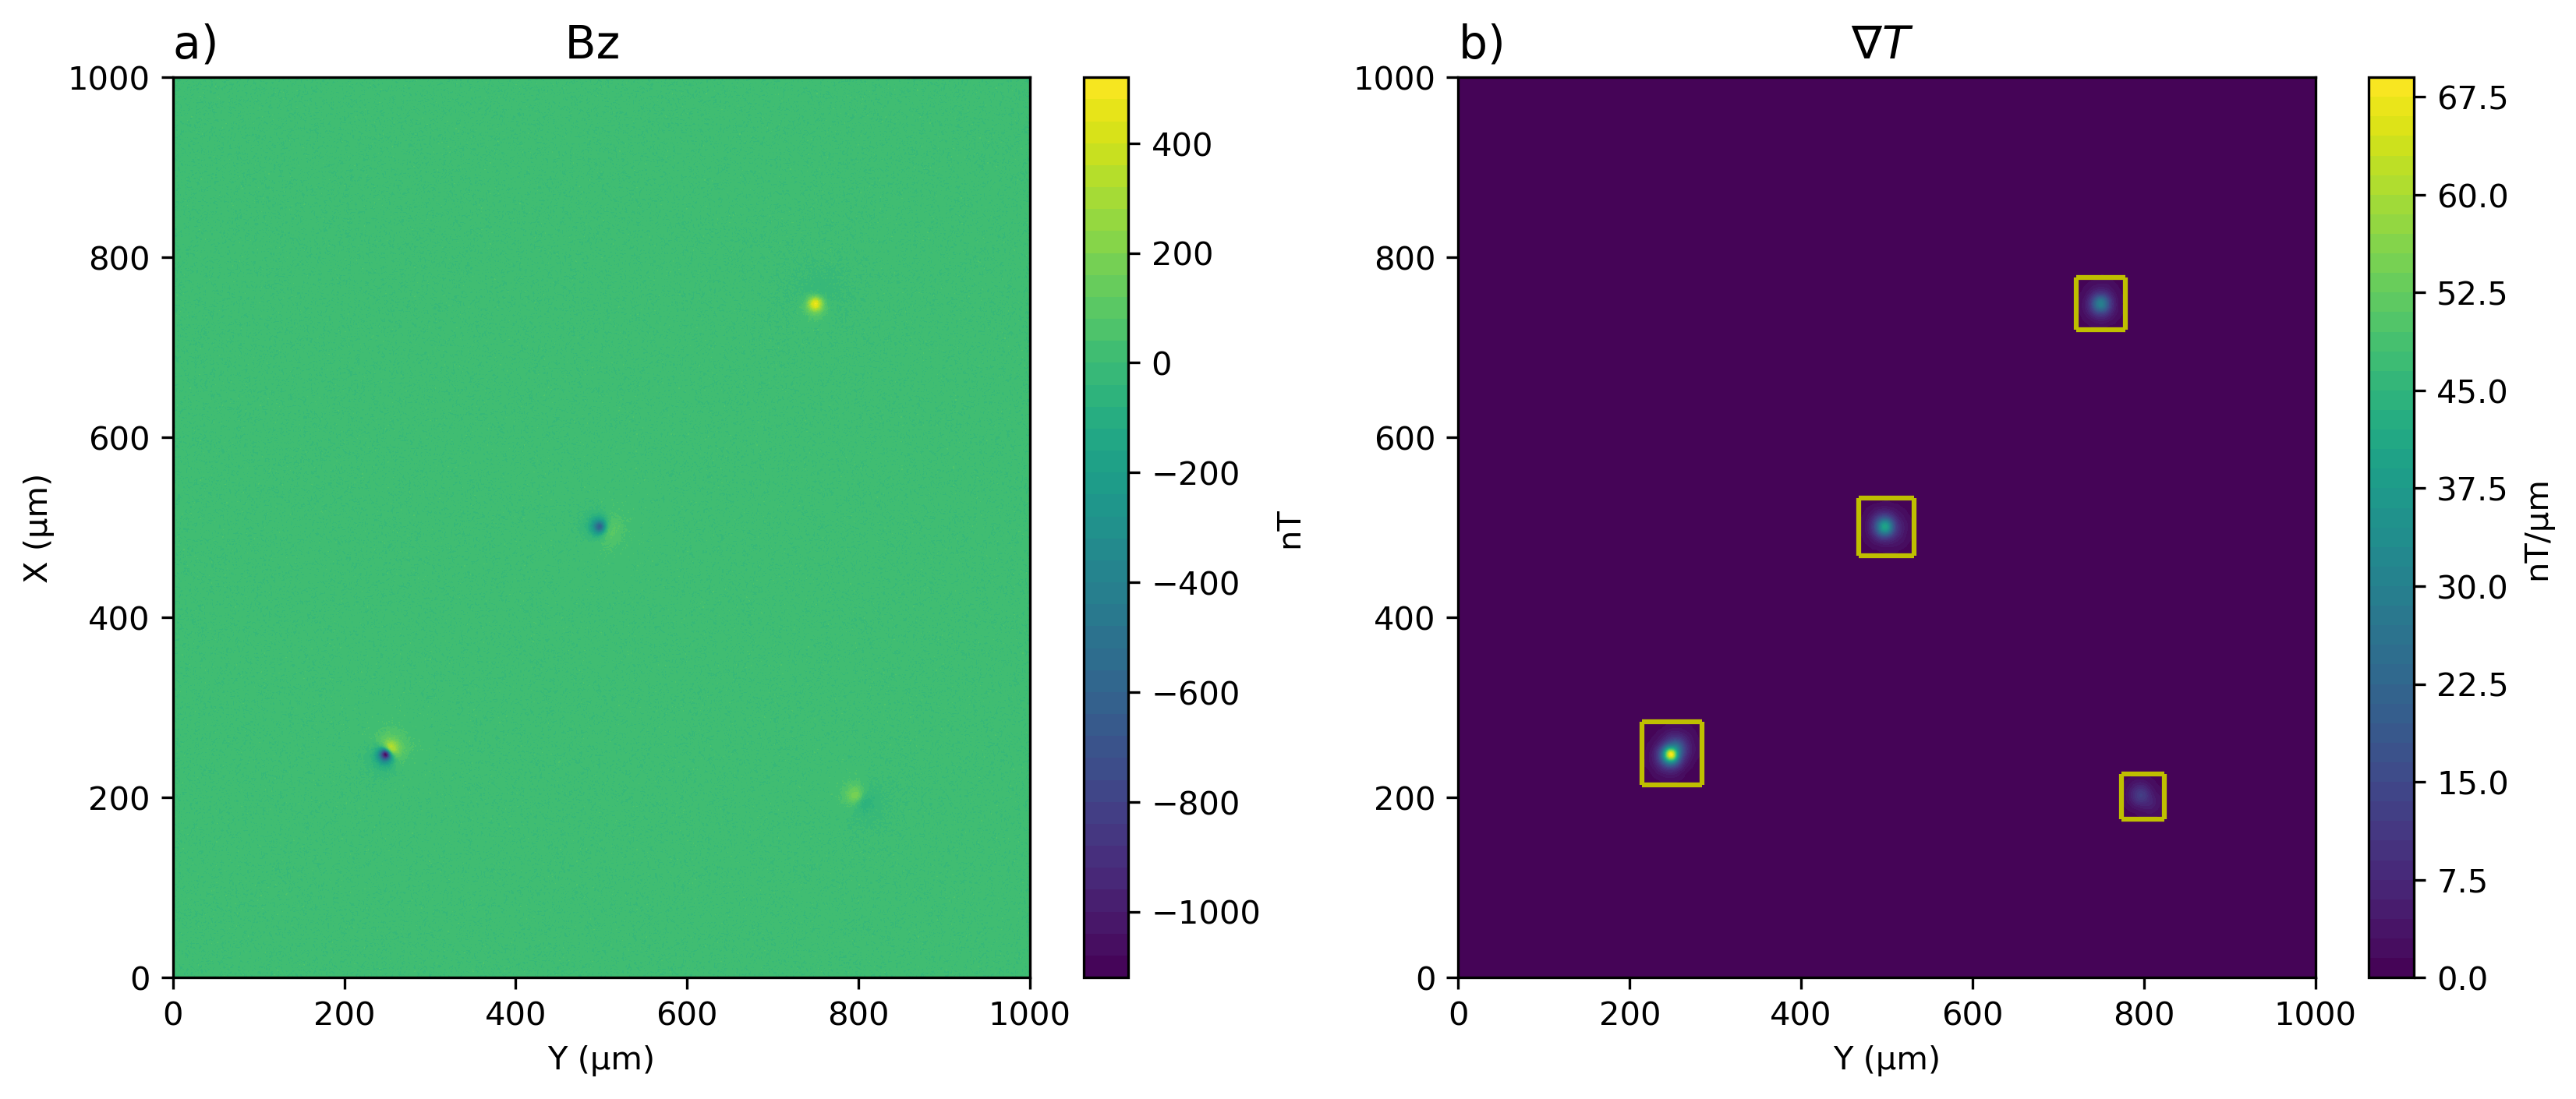
\includegraphics[width=1.0\textwidth]{SimpleSynthetic.png}
\caption{a) Synthetic data contaminated with psedo-random normal noise. b) Individual sources window position (yellow squares) obtained with the blob detection algorithm applied on the total gradient map.}
\label{fig:SimpleSynthetic}
\end{figure}


\noindent{After isolating the potencial field data and first derivatives for each source, we can solve the 3D Euler deconvolution \cref{eq:euler2} proposed by  \cite{Reid1990}, one for each subarea selected (window data), by assuming the structural index of a sphere/punctual source ($n = 3$). Thus, obtaining a sturdy result for the central positioning (Xc, Yc, Zc) of each source causing the magnetic potential anomaly in the observed data set, as shown in \cref{tab:SimpleSyntheic}.}

\noindent{The last step consists of using the central positions of each source, obtained with Euler's method, as an input parameter for inverting the original noisy data (\cref{fig:SimpleSynthetic}a) to find the least squares (or robust) approximation solution for the vector of cartesian magnetic moments ($\bar{m}$). With this, the magnetization directions (D and I) and the intensity of the magnetic moment can be estimated using equations (\cref{eq:sphere16,eq:sphere17,eq:sphere17_m}), as well as the uncertainty propagation of this inversion, using equations (\cref{eq:sphere21,eq:sphere22,eq:sphere22_m}) and considering $\sigma$ = 25nT. The results obtained with the least squares estimator can also be seen in \cref{tab:SimpleSyntheic}.}

\noindent{It is important to emphasize that \cite{OliveiraJr.2015} proved that the magnetization directions (D and I) recovered by the least squares estimator is sensitive to variations in the horizontal coordinates (x and y) of the magnetic sources central positions. While, the same being practically insensitive to variations in depths. Thus, the same authors consider Euler deconvolution method as an adequate technique to estimate the central positions that will be used as a priori information for inversion. This occurs mainly because, when well performed, the recovery of the horizontal coordinates of sources central position is considerably accurate, while the vertical coordinate can undergo greater variation \citep{Silva2003, Melo2013}, even so the inversion will still provide extremely satisfactory results. The high sensitivity of Euler deconvolution to high frequency noise can also be easily overcome with the proper application of the upward continuation filter.}


\subsection{Complex Simulation: Testing Applicability}

\noindent{This test tries to replicate a more complicated scenario by simulating a hundred sources randomly distributed in the imaged area of ​​the synthetic thin section of 2000 x 1400 $\mu m$, with 2 $\mu m$ grid spacing and 5 $\mu m$ sample-sensor distance. For greater fidelity with real samples, the magnetic sources have different diameters, magnetizations and depths. The depths of the spheres vary between 1 and 19 $\mu m$, while the radii have values ​​that range from 0.01 to 0.95 $\mu m$. The magnetization acquisition simulates an induced field with both declination and inclination directions of 45\textdegree. However, as seen in real data, these directions have both varying declination and inclination, but averaging centered in the direction of the induced field. Therefore, both the NRM declination and inclination of the particles were selected using pseudo-random normal distribution with mean 45\textdegree and standard deviation of 8\textdegree. Finally, high (pseudo-random normal with zero mean and standard deviation of 5 nT) and low frequency noises were added to the anomaly data of the vertical field component of the magnetic field, which can be seen in \cref{fig:ComplexSynthetic}a.}

\noindent{After applying the same filtering steps described earlier on the simple synthetic sample, the blob detection algorithm was applied on the total gradient anomaly map and the individual source windows were selected (\cref{fig:ComplexSynthetic}b). The latter was able to detect 84 magnetic particles. The solution of Euler's equation was then determined for each data window to later be used as input data for inversion of magnetic moments.}

\begin{figure}[hbpt]
\centering
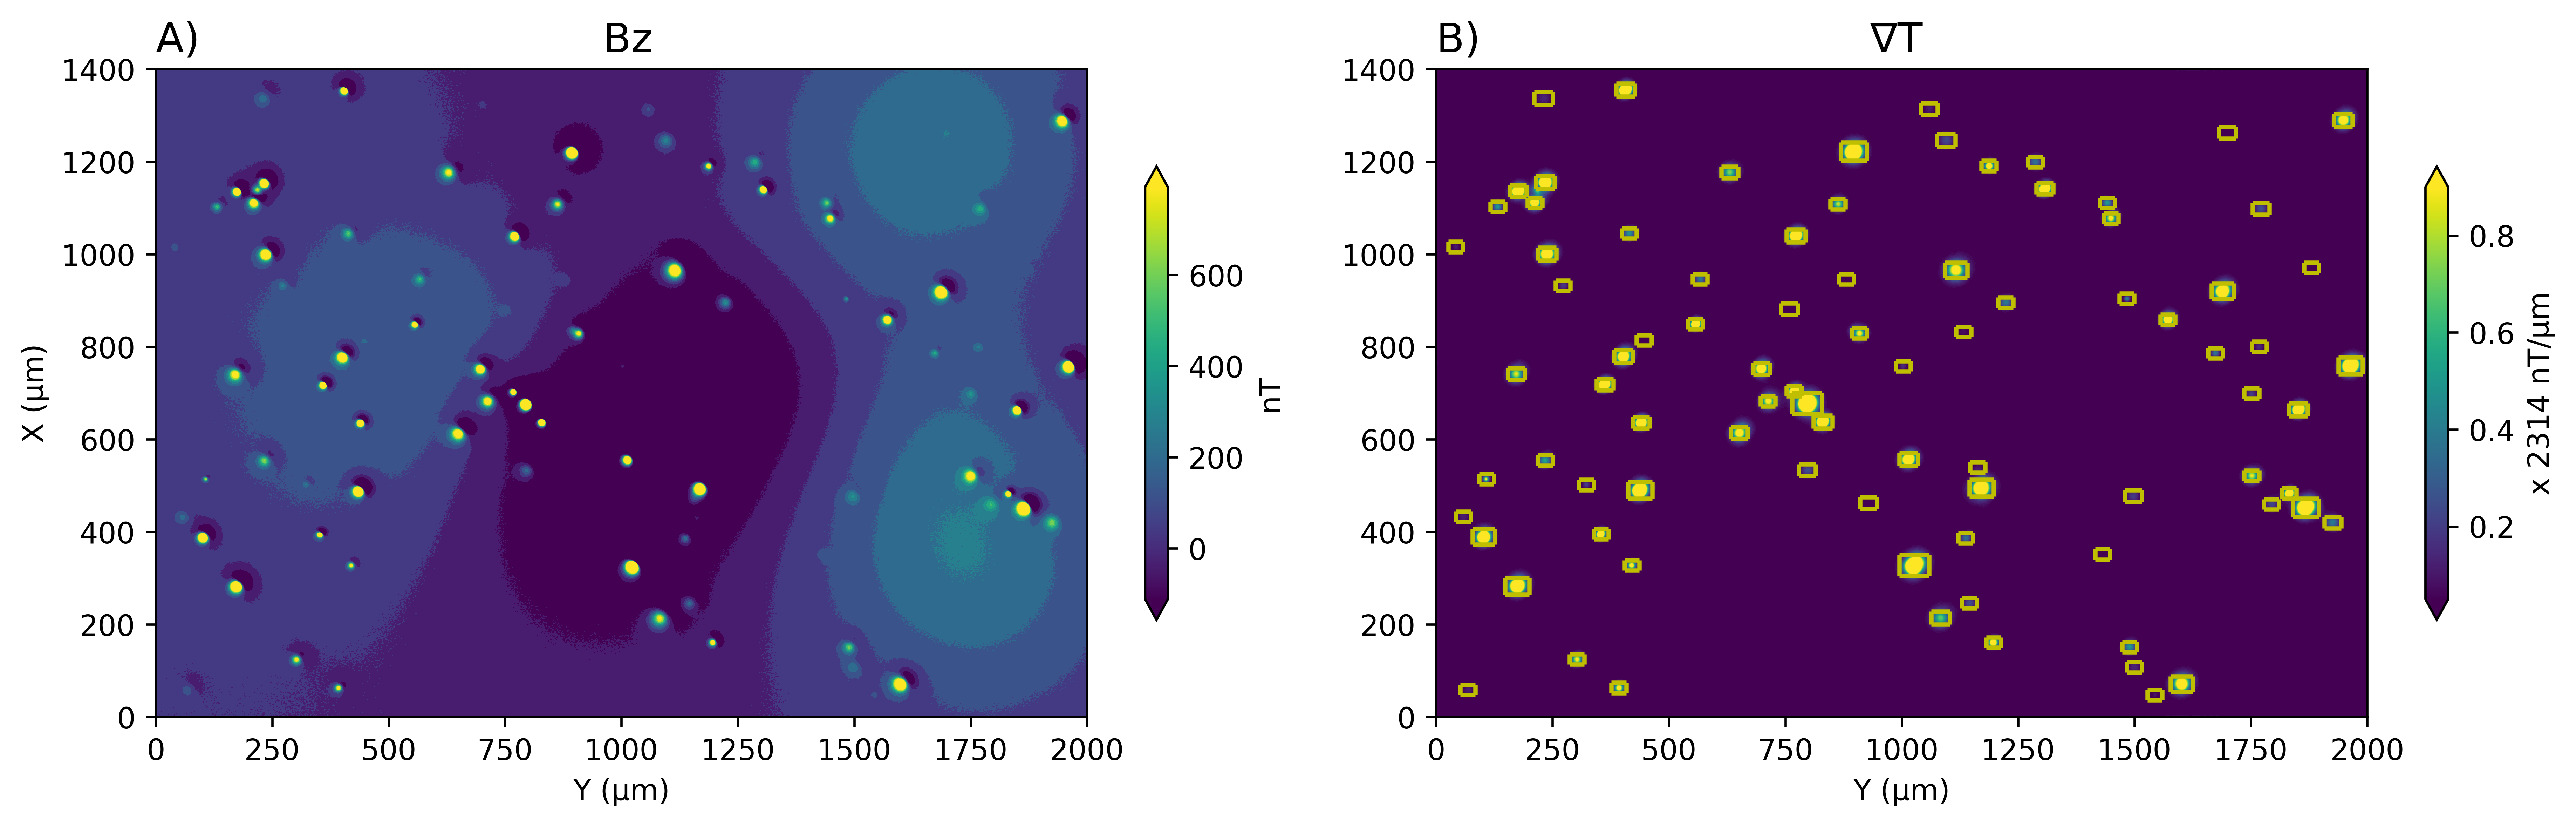
\includegraphics[width=1.0\textwidth]{ComplexSynthetic.png}
\caption{a) Complex synthetic data contaminated with  both high and low frequencies noise. b) Individual sources window position (yellow squares) obtained with the blob detection algorithm applied on the total gradient map.}
\label{fig:ComplexSynthetic}
\end{figure}

\noindent{The spatiality of the inversion results is one of the great differences between the application of magnetic microscopy and the classic techniques of paleomagnetism. Thus, the validation of these results is expressed individually in the windows obtained with the blob detection through the declination, inclination and magnetic moment misfits (\cref{fig:ComplexSynthetic2}a-c, respectively), in addition to the determination coefficient R$^2$ obtained by comparing the forward model and the observed data (\cref{fig:ComplexSynthetic2}d). As both the depth and the size of the particles influence the magnetic signal generated by them, this information is also given in these graphs in the form of a cross bar. Where the vertical bars scale with the depth of the sources (max = 19 $\mu m$), while the horizontal bars scale with the radius (max = 0.95 $\mu m$).}

\begin{figure}[hbpt]
\centering
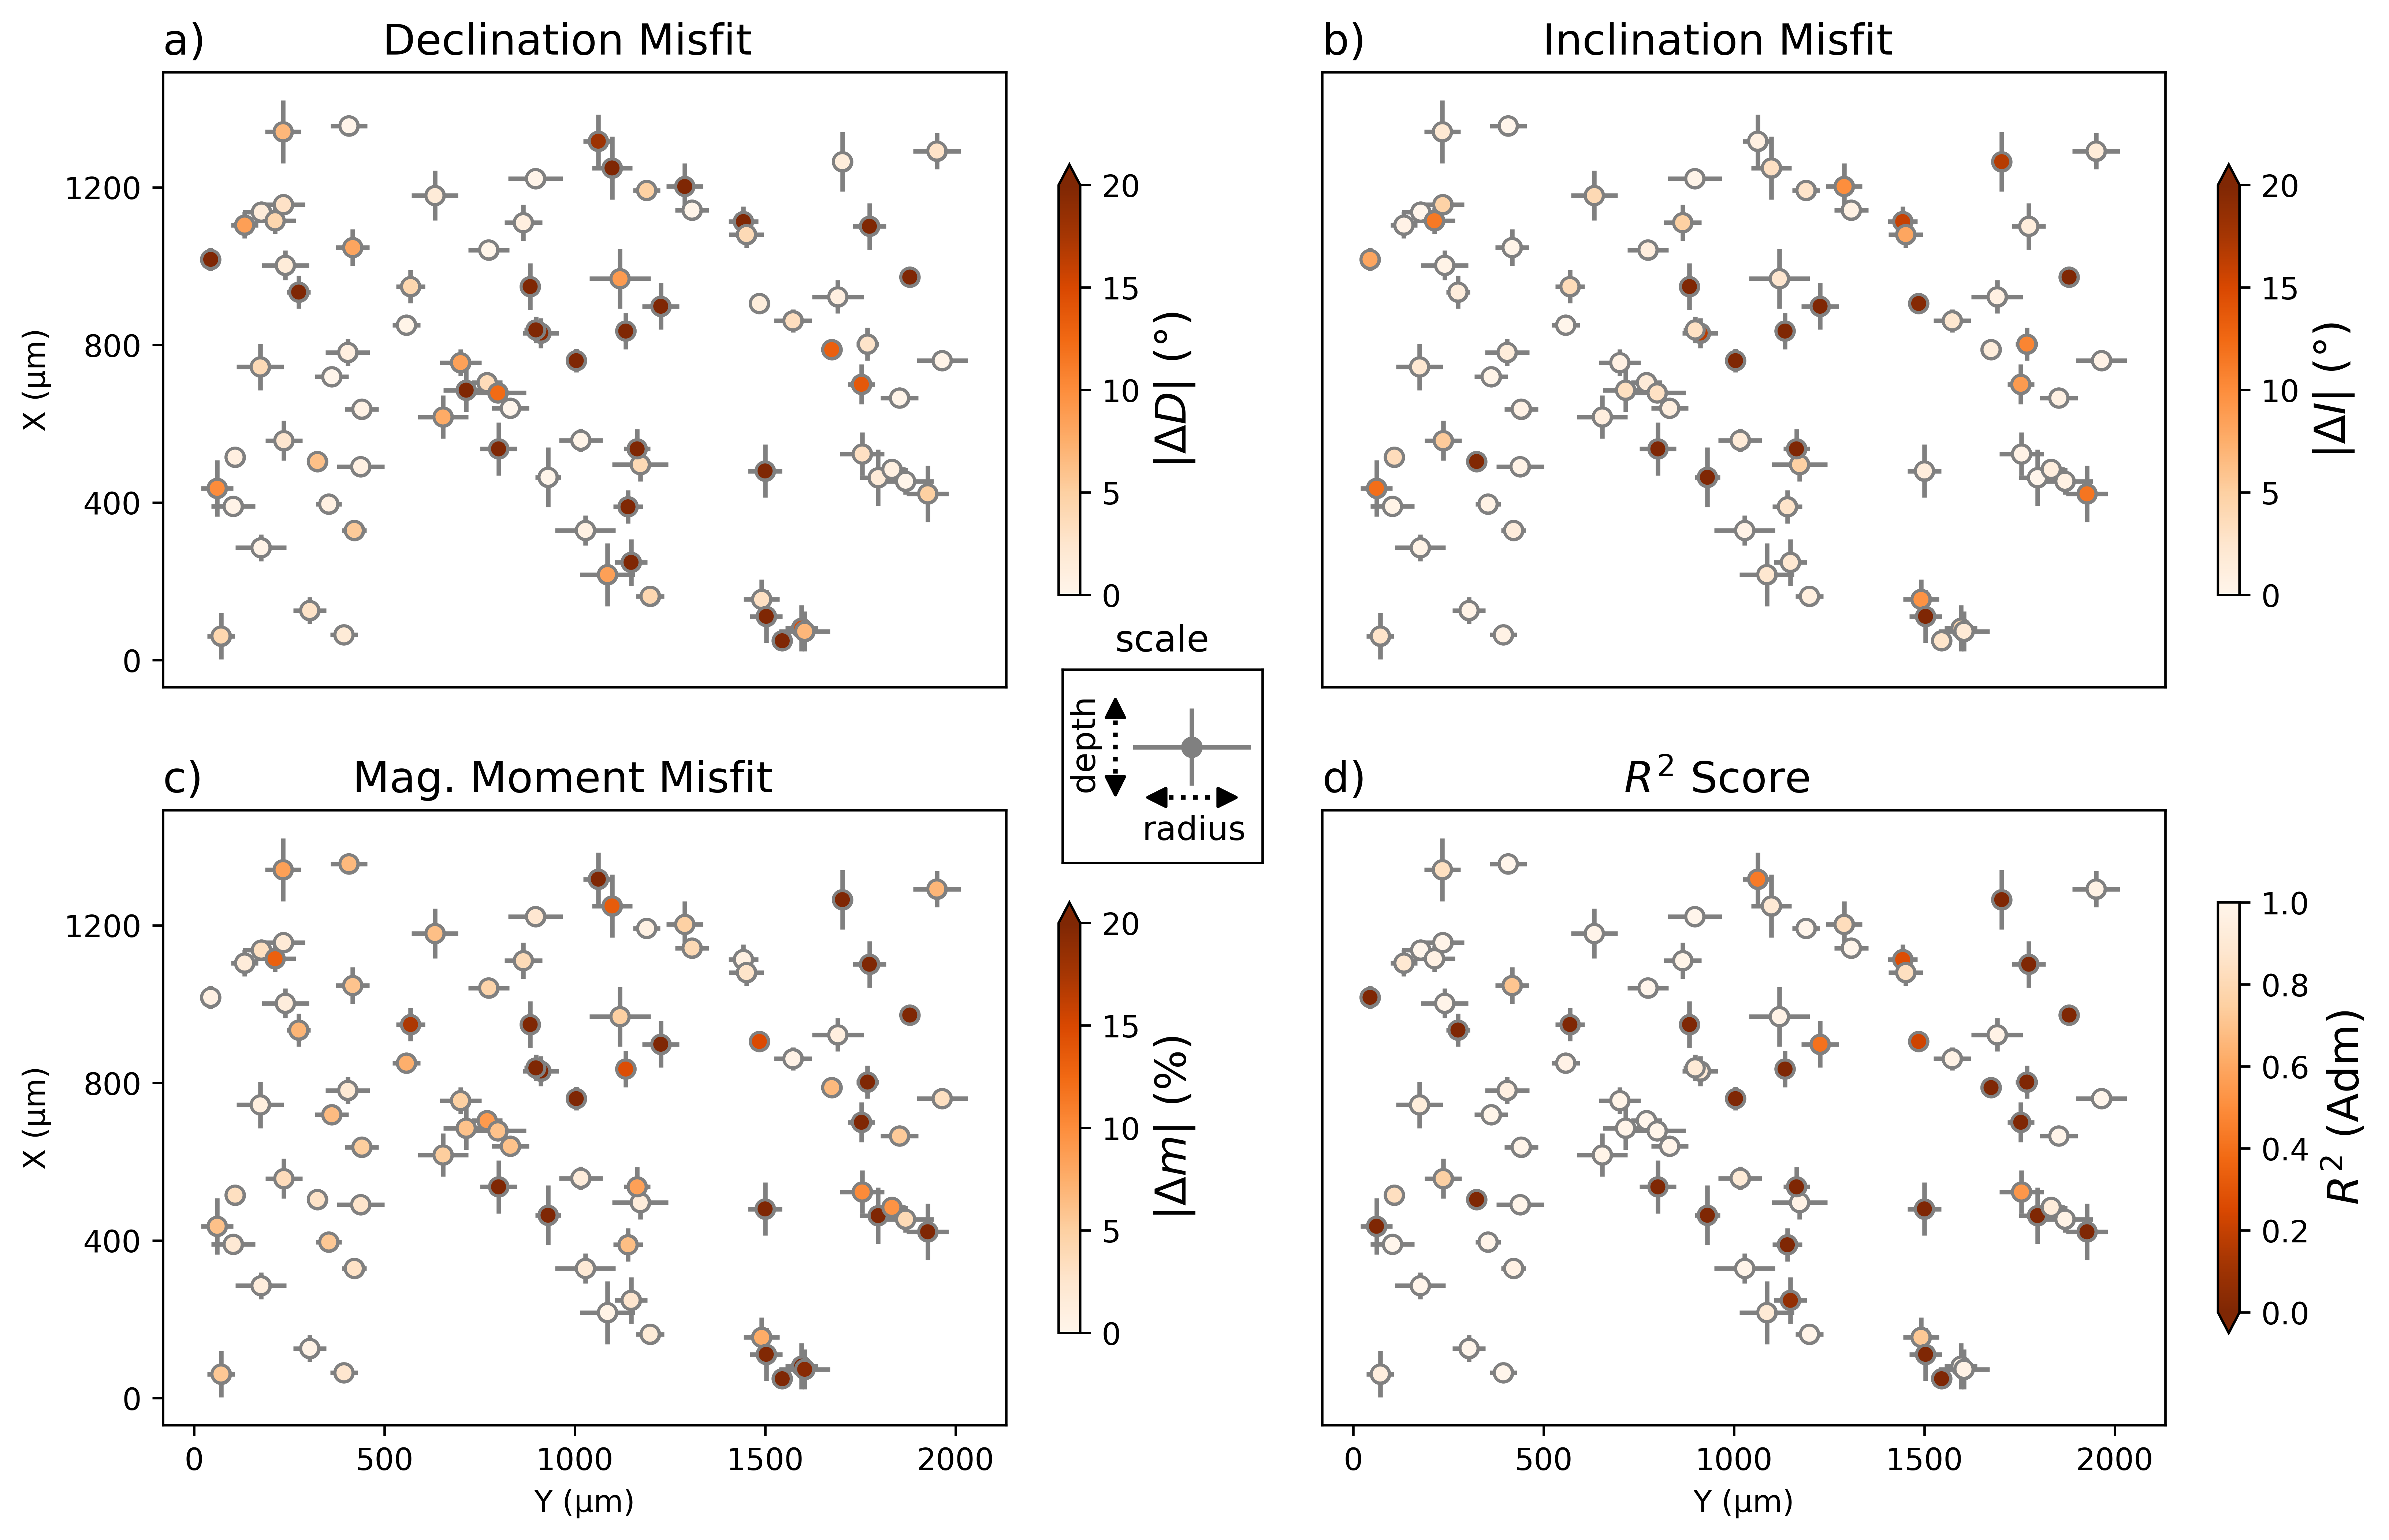
\includegraphics[width=1.0\textwidth]{ComplexComparison.png}
\caption{The validation of the result obtained with the inversion was calculated for each individual particle based on the error between the real parameters modeled and their respective recovered values, being directions of (a) declination and (b) inclination and (c) intensity of magnetic moment , in addition to the R$^2$ score (d) obtained by comparing the forward model and the actual data. The depth and radius of the magnetic sources are also important factors that influence the final result, therefore, these data are given in the form of cross plots, with the vertical bar represented by the depth (1 - 19 $\mu m$) and the horizontal bar by the radius (0.01 - 0.95 $\mu m$).}
\label{fig:ComplexSynthetic2}
\end{figure}

\noindent{The application in complex synthetic data also allows observing the strengths and limitations of the proposed methodology. Some of the strengths that can be mentioned are: (i) the fact that the applied technique not only detects most of the modeled sources, but also (ii) most of the recovered magnetic parameters have considerably low errors, especially in the declination and inclination directions, usually less than 5\textdegree (\cref{fig:ComplexSynthetic2}a-b). (iii) The magnetic moments obtained also tend to not deviate much from the real values (\cref{fig:ComplexSynthetic2}c) when the R$^2$ scores are high (\cref{fig:ComplexSynthetic2}d). (iv) Shallow particles grouped in clusters are usually well individualized during window selection, as well as (v) some weak signal but isolated particles.}

\noindent{While, the limitations observed were already expected, namely (i) the blob detection is insensitive when there are sources that are very close, grouping them in the same window, thus causing an erroneous result both for Euler deconvolution and for the magnetic parameters. (ii) The very same occurs when there is a source under another, in this case the magnetic signal is a sum of both. (iii) In clusters of larger and/or deeper particles, although the method individualizes them well, the magnetic signal of the neighboring particles can considerably influence the result of the inversion}

\noindent{Apparently there is a direct relationship between the vertical position and depth with the observed errors. It is clear from cross bars on the \cref{fig:ComplexSynthetic2} that deep particles and/or with small radii generate worse results than those more superficial particles with larger radii, this is mainly because these two properties will influence the signal picked up by the sensor. Small particles have weaker magnetic moment signal, in addition, very deep sources have their signal considerably attenuated at the height of the sensor, when both characteristics are present at the same time the error tends to be greater. The opposite is also true, larger particles and superficial particles have their signal better captured by the sensor. Small and superficial particles might also generate low errors because, despite having lower magnetic moments, the sensor-sample distance is sufficient to generate a good signal.}

\noindent{The modeled magnetization directions not only generate an average direction coincident with the simulated induced field, but also have relatively small Fisher cones of confidence \citep{Fisher1987} due to their clustering (\cref{fig:ComplexSynthetic3}a). On the other hand, the recovered directions may be more sparse, despite this the mean direction obtained is statically the same as the field modeled inside the 95\% confidence cone (\cref{fig:ComplexSynthetic3}b). If necessary, the data can be filtered according to the highest adjustments obtained with the coefficient of determination (R$^2$). The value of R$^2$ can vary from $-\infty$ to 1, with values closest to 1 corresponding to the best modeling results. Thus, filtering the results obtained with the magnetic inversion with R$^2 \geq 0.7$ we obtain the directions closest to the average and less sparse, maintaining the high reliability result (\cref{fig:ComplexSynthetic3}c).}

\begin{figure}[hbpt]
\centering
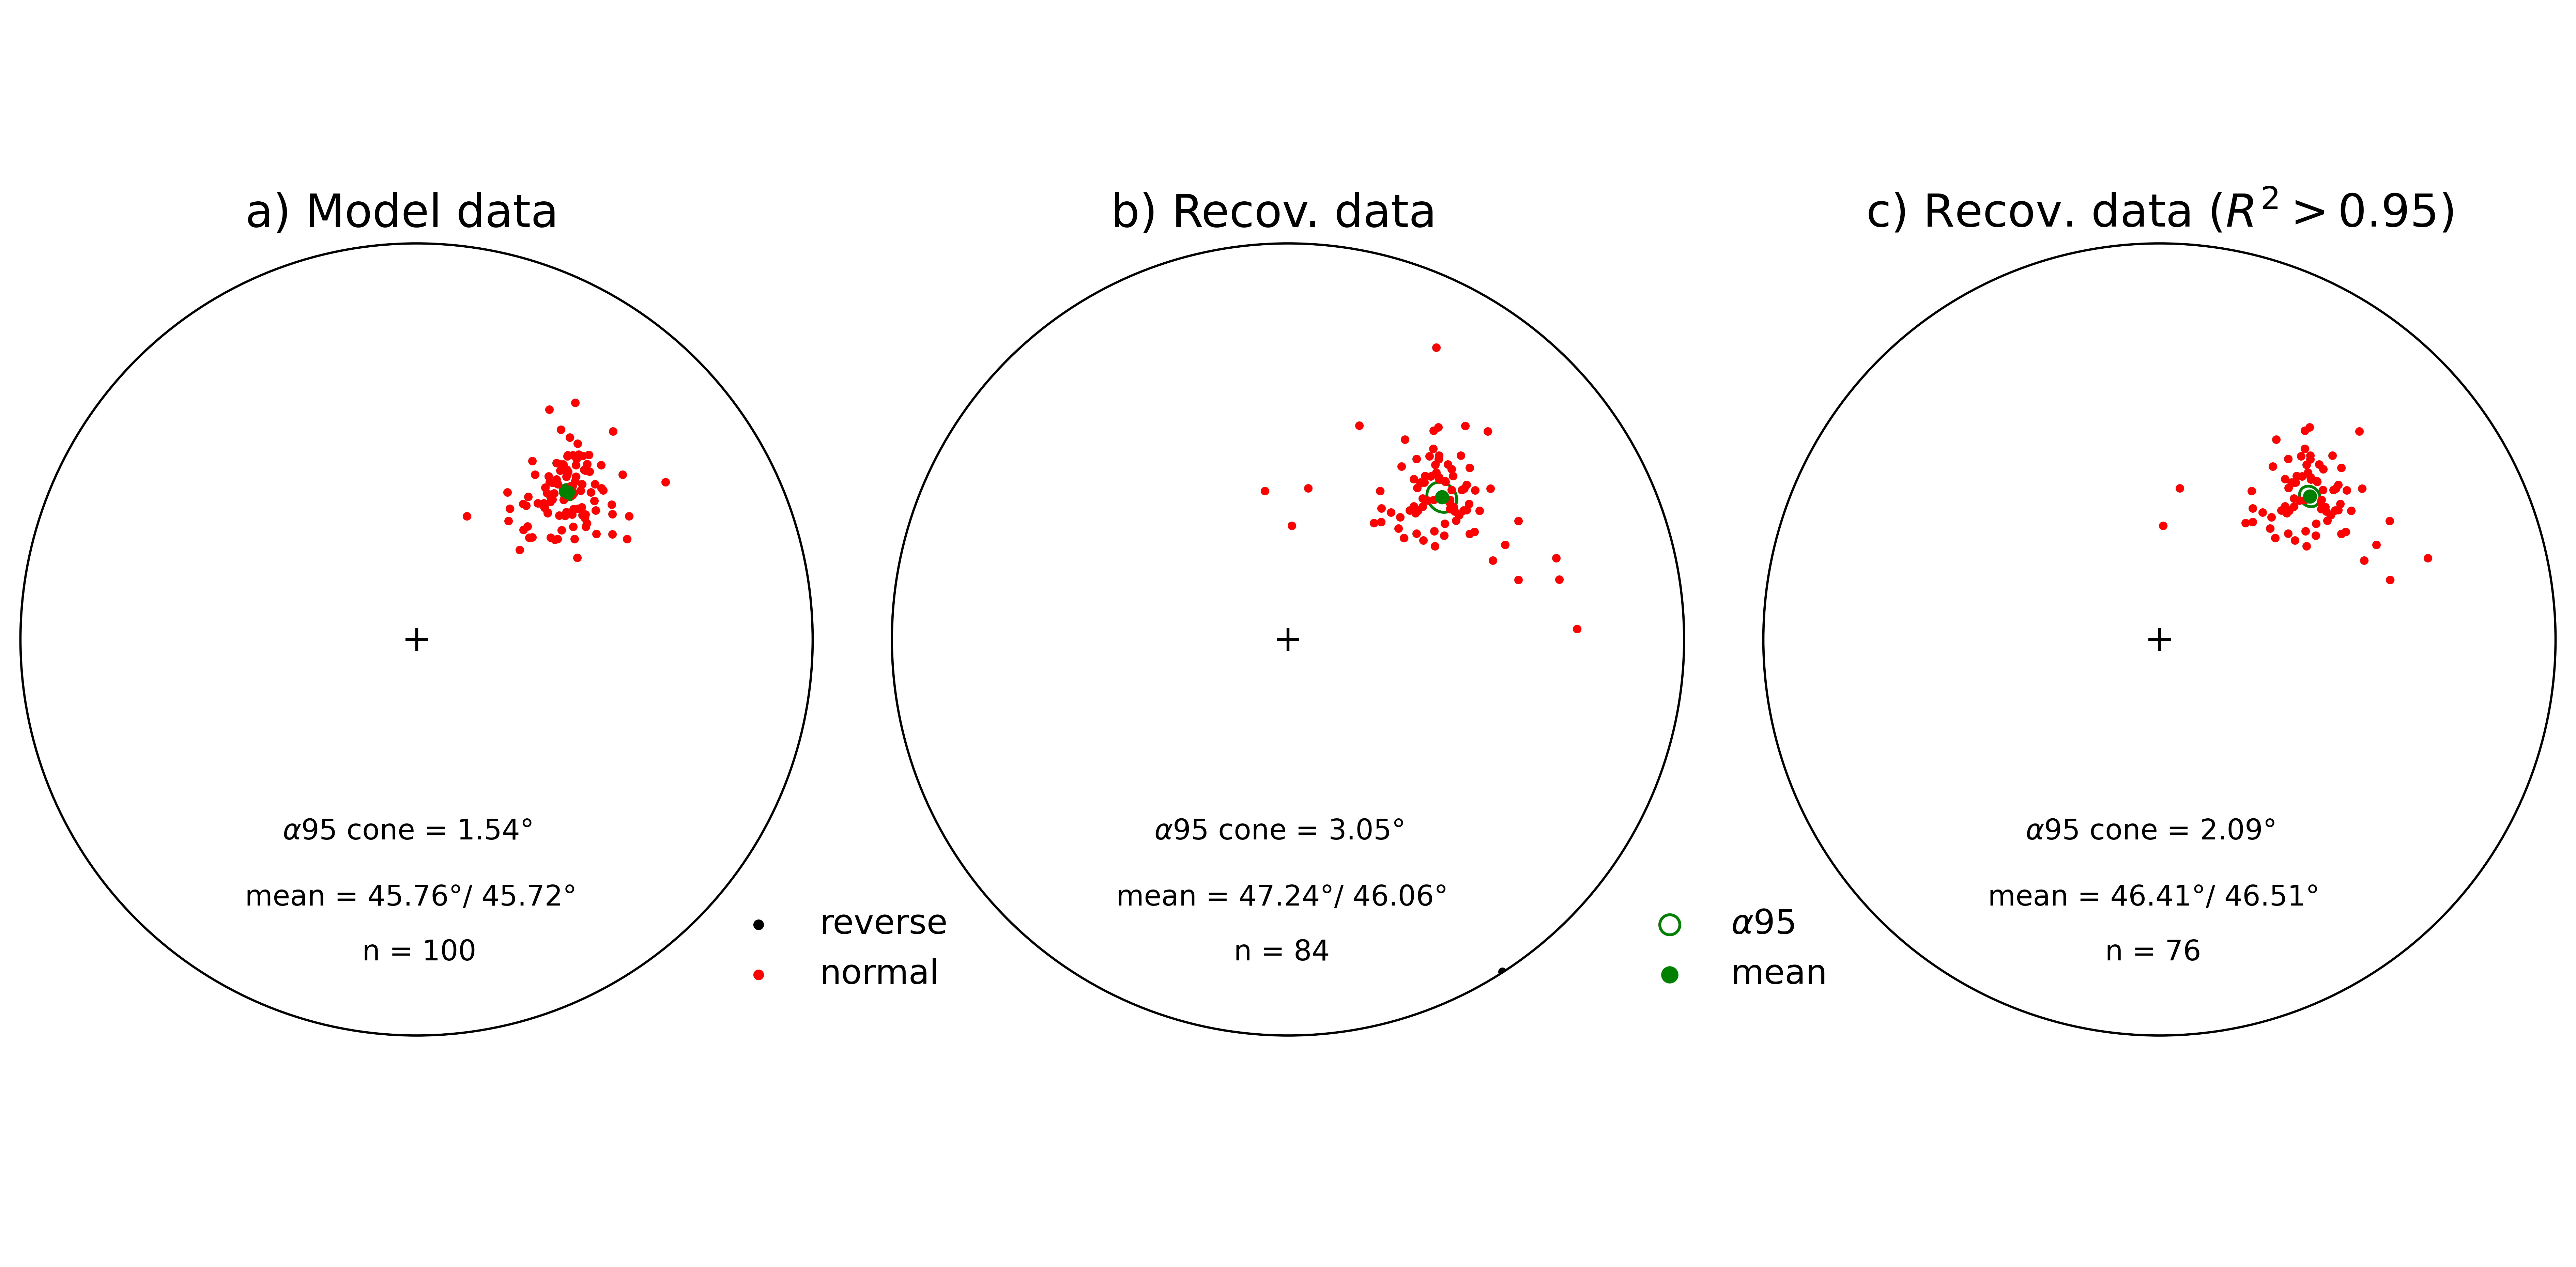
\includegraphics[width=1.0\textwidth]{ComplexStereo.png}
\caption{a) The real data models a thin section of rock with particles uniformly magnetized in the average direction of the induced field 45\textdegree/45\textdegree. b) The recovered data, without any type of filtering, are sparse, but statistically generate the same average direction. (c) It is still possible to filter only the directions of the magnetic sources with the best fitting determined by the coefficient of determination (e.g., $R^ 2 \geq 0.7$) to ensure better grouping of the directions around the mean value.}
\label{fig:ComplexSynthetic3}
\end{figure}

\end{singlespace}